\documentclass{beamer} %para presentación
\usepackage{graphicx}
\usepackage[utf8]{inputenc}
\usepackage[spanish]{babel}
\graphicspath{{Imagenes/}}
%\usetheme{Antibes} %es para cambiar el tema
%\usetheme{AnnArbor}
%\usetheme{Berkeley}
%\usetheme{CambridgeUS}
%\usetheme{Goettingen}
%\usetheme{Bergen}
%\usetheme{Dresden}
%\usetheme{Boadilla}
%\usetheme{sidebar}
\usetheme{Darmstadt}
\title{Taller de Herramientas Computacionales}
\author{Stephanie Escobar Sánchez}
\date{22-enero-2019}

%esto se utiliza para el tema
%\def\insertauthorindicator{¿Quién?}
%\def\insertdateindicator{Fecha}

\begin{document}
	\maketitle
	
\begin{frame}
	\frametitle{Mi primera diapositiva}
	\begin{center}
		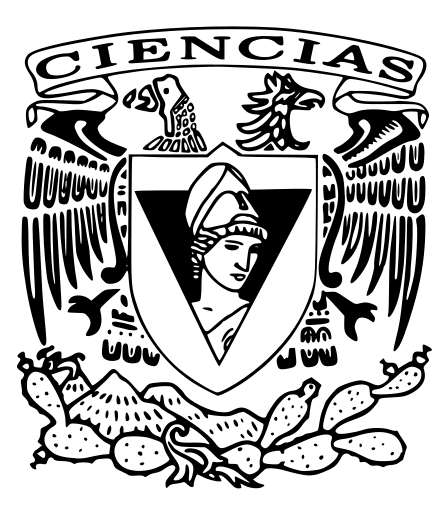
\includegraphics[scale=0.5]{1.png}
	\end{center}
		
\end{frame}

\begin{frame}

\transboxin

\frametitle{Segunda diapositiva}
Esta es mi segunda diapositiva

\end{frame}
\begin{frame}[fragile]
	\begin{verbatim}
#!/usr/bin/python2.7
# -*- coding: utf- 8 -*-

print 'Hoy es miércoles'
'''
Stephanie Escobar Sánchez, 311210666
Taller de herramientas computacionales
Este es un programa que dice 'Hoy es miércoles'

'''

x = 10.5; y = 1.0/3; z = 15
#x, y, z = 10.5,1.0,15.3 (otra forma)

H= """
El punto en R3 es:
(x, y, z) = %.2f, %g, %G)
""" % (x, y, z)
print H

G= """
El punto en R3 es:
(x, y, z) = ({laX: .2f}, {laY:g}, {laZ:G})
""" .format (laX=x, laY=y, laZ=z)
print G

import math as m
from math import sqrt
from math import sqrt as s
x = input("¿Cuál es el valor al que le quieres calcular la raíz cuadrada?")
		print "la raiz cuadrada de %.2f es es %f" % (x, m.sqrt(x))
			print sqrt (4)
print s(16.5)

	\end{verbatim}

\end{frame}

\end{document}

